\chapter{Heat equation -- 2D -- Temperature field of an L-shaped domain}

\modinfo{Directory}{TemperatureAngleGUI}
\modinfo{Solvers}{\Idx{HeatSolve}} 
\modinfo{Tools}{\Idx{ElmerGUI}} 
\modinfo{Dimensions}{2D, Steady-state}
\modinfo{Author}{Peter R{\aa}aback}


\subsection*{Problem description}

An L-shaped structure 
(see figure~\ref{fg:struct1}) 
is heated by an
internal heat source, which magnitude is 1 W/m$^3$. The density of the
structure is 1 kg/m$^3$ and the heat conductivity is 1 W/mK. All the
boundaries $\Gamma_i$ are kept on constant temperature of 0 K. The
problem is to solve the temperature distribution in the structure.
Mathematically the problem to be solved is
\begin{equation}
\left \{
\begin{array}{cccc}
- \kappa \Delta T &= &\rho f & \mathrm{ in } \Omega \\
T&=&0 & \mathrm{ on } \Gamma
\end{array}
\right .
\end{equation}
where $\kappa$ is the heat conductivity, $T$  is the temperature 
and $f$ is the heat source. It is assumed that density 
and heat conductivity are constants. 
\begin{figure}
\begin{center}
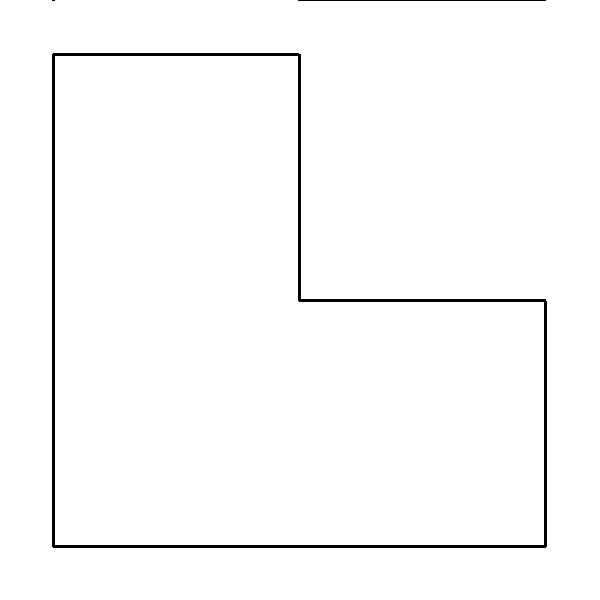
\includegraphics[width=50mm, viewport=20 20 580 580,clip]{angle}
\caption{L-shaped domain}\label{fg:struct1}
\end{center}
\end{figure}

\subsection*{Solution procedure}

Start \texttt{ElmerGUI} from command line or by clicking the icon in your desktop. Here we describe 
the essential steps in the ElmerGUI by writing out the clicking procedure. Tabulation generally means that the selections are done within the window chosen at the higher level. 

The mesh is given in ElmerGrid format in file \texttt{angle.grd} in the samples directory of ElmerGUI, 
load this file.
\ttbegin
File 
  Open -> angle.grd
\ttend
You should obtain your mesh and may check in the \texttt{Model summary} 
window that it consists of 341 nodes and 300 bilinear elements.
If the mesh was successfully imported your window should look something in figure~\ref{fg:mesh1}.

\begin{figure}
\begin{center}
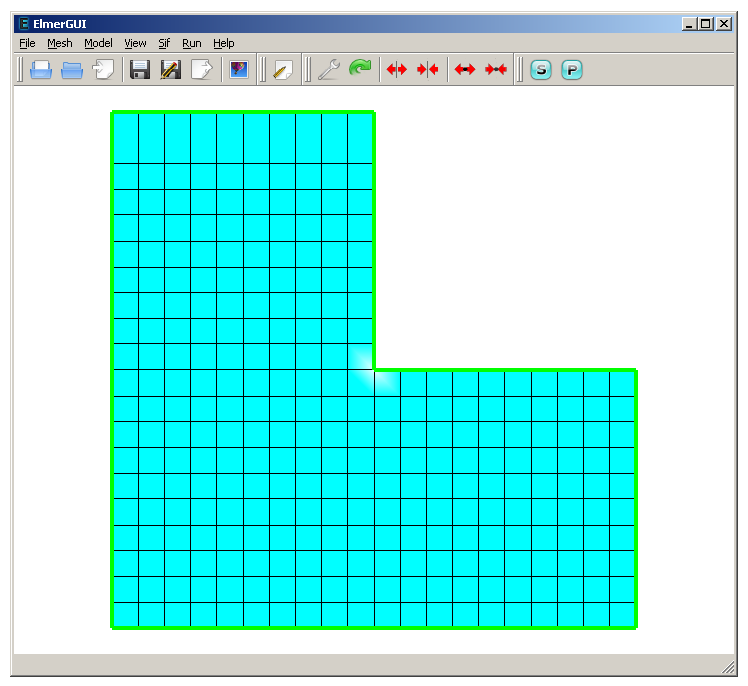
\includegraphics[width=100mm]{Tangle_mesh}
\caption{The finite element mesh in ElmerGUI}\label{fg:mesh1}
\end{center}
\end{figure}

After we have the mesh we start to go through the Model menu from the top to bottom. 
In the \texttt{Setup} we choose things related to the whole simulation such as file names, 
time stepping, constants etc.
The simulation is carried out in 2-dimensional Cartesian
coordinates and in steady-state. 
Only one steady-state iteration is needed as the case is linear. 
\ttbegin
Model
  Setup 
    Simulation Type = Steady state
    Steady state max. iter = 1
\ttend
Choose \texttt{Accept} to close the window.

In the equation section we choose the relevant equations and parameters related to their solution. 
In this case we'll have one set only one equation -- the heat equation.


When defining Equations and Materials it is possible to assign to the bodies immediately, or to use mouse
selection to assign them later. In this case we have just one body and one boundary and therefore its easier to assign 
the Equation and Material to it directly.

For the linear system solvers we are happy to use the defaults. One may however, try out different
preconditioners (ILU1,\ldots) or direct Umfpack solver, for example.
\ttbegin
Model
  Equation
    Add 
      Name = Heat Equation
      Apply to bodies = 1
      Heat Equation
        Active = on
  Apply   
  OK
\ttend        

The Material section includes all the material parameters.
They are divided into generic parameters which are direct properties of the material
without making any assumptions on the physical model, such as the mass. Other properties assume
a physical law, such heat conductivity.
\ttbegin
Model
  Material
    Add 
      Name = Ideal
      Apply to bodies = 1 
      General    
        Density = 1.0
      Heat Equation
        Heat Conductivity = 1.0
    Apply
    OK
\ttend

A Body Force represents the right-hand-side of a equation that in this case represents
the heat source. 
\ttbegin
Model
  Body Force
    Add 
      Name = Heating
      Heat Source = 1.0
      Apply to bodies = 1
    Apply
    OK
\ttend    

No initial conditions are required in steady state case.

In this case we have only one boundary and set it to zero.
\ttbegin
Model
  BoundaryCondition
    Add 
      Heat Equation
        Temperature = 0.0
      Name = Zero
      Apply to boundaries = 1
    Apply
    OK
\ttend   


For the execution 
ElmerSolver needs the mesh files and the command file. We have now basically defined
all the information for ElmerGUI to write the command file. After writing it we may also visually 
inspect the command file.
\ttbegin
Sif 
  Generate
  Edit -> look how your command file came out  
\ttend

Before we can execute the solver we should save the files in a directory. In saving the project all the
necessary files for restarting the case will be saved to the destination directory.
\ttbegin
File 
  Save Project
\ttend

After we have successfully saved the files we may start the solver
\ttbegin
Run
  Start solver
\ttend
A convergence view automatically pops up showing relative changes of each iteration.
As the case is linear only one iteration was required for the solution and the second one
just is needed to check the convergence. 
The resulting output log is shown in figure~\ref{fg:log1}.

\begin{figure}
\begin{center}
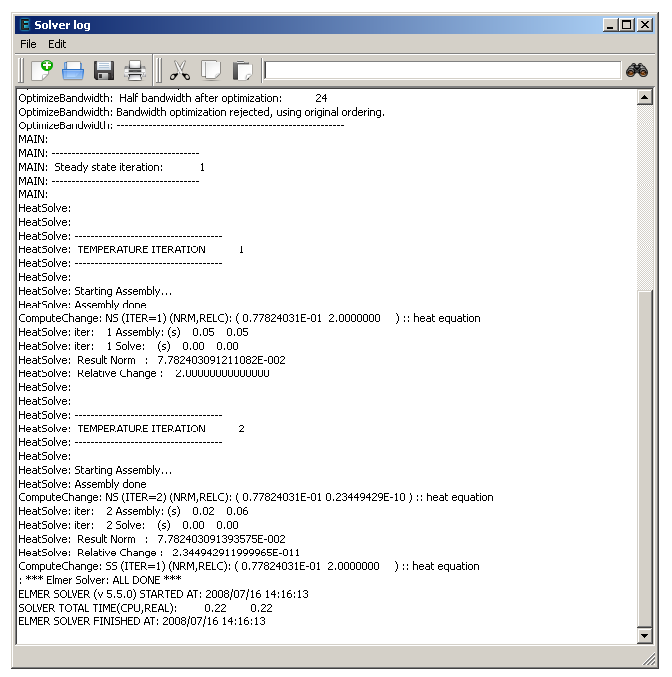
\includegraphics[width=100mm]{Tangle_com}
\caption{The output log of ElmerSolver when used under ElmerGUI}\label{fg:log1}
\end{center}
\end{figure}

Note: if you face problems in the solution phase and need to edit the setting, always remember to save
the project before execution.

To view the results we use Paraview.
\ttbegin
Run
  Start Paraview
\ttend
Picture~\ref{fg:post1} shows the the surface mesh colored with temperature (the pictures were
generated by the obsolete ElmerPost software).

\begin{figure}
\begin{center}
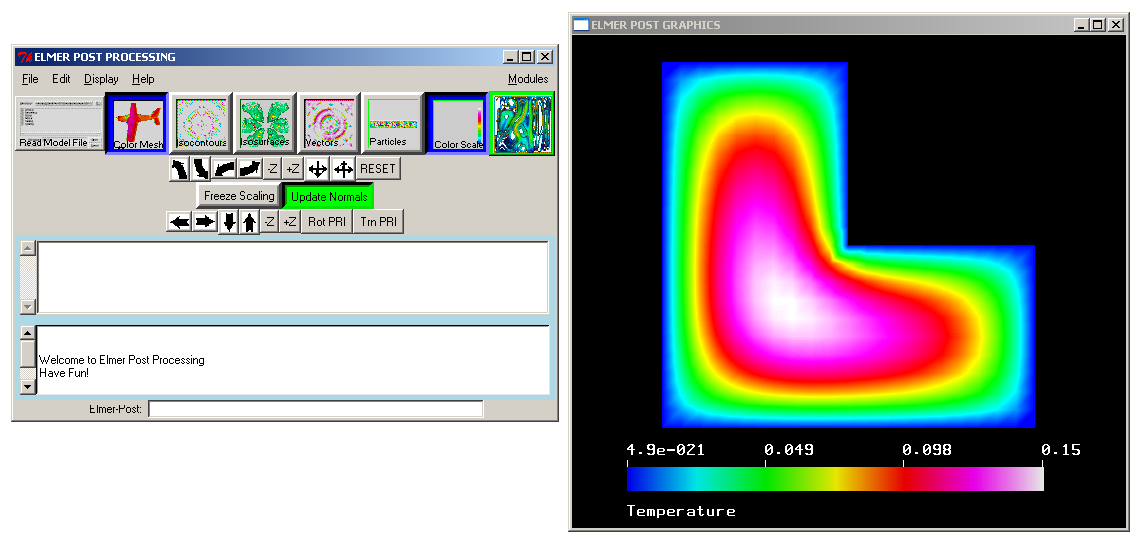
\includegraphics[width=140mm]{Tangle_post}
\caption{The temperature distribution of the L-shaped domain.}\label{fg:post1}
\end{center}
\end{figure}


\subsection*{Results}

As a reference result the maximum temperature in the structure is given. For a
comparison the same problem was solved six times with different
element sizes using the \texttt{-relh} flag of \texttt{ElmerGrid} format located in the
\texttt{Mesh} menu under \texttt{Configure}. After choosing \texttt{Remesh} and saving the mesh 
the solver may be recalled with the modified mesh.

The maximum temperature obtained by using different
meshes is recorded in Table~\ref{tb:res1}.  From the results one
can see that the result converges. With a denser mesh the result is
more accurate, but solving the problem takes more calculation time.
For reference, the CPU-time used in each case is
also shown in the table (using Lenovo 60 laptop).

\begin{table}[h]
\caption{Results with different element sizes}
\label{tb:res1}
\begin{center}
\begin{tabular}{llll} \hline
Model mesh h [m] & Elements & $\max (T)$ [K] & cpu time [s]\\ \hline
0.2 & 75 &  0.1452  & 0.14 \\
0.1 &  300 & 0.1477  & 0.19 \\
0.05 & 1200 & 0.1489  & 0.41 \\ 
0.025 & 5120 & 0.14925 & 1.22 \\ 
0.01  & 30800 & 0.14937 & 7.77 \\ \hline
\end{tabular}
\end{center}
\end{table}

\hfill
\mbox{}






